We extracted nine sets of features for each cohort, labeled as F1 through F9.  Specifically, 
the first three sets are based on patient demographics and are meant to be used as null models. The remaining six sets consist of radiomics-based features similar to Shu et al.'s original sets (See Fig~\ref{featureExtraction}).

\begin{figure}[!ht]
  \centering
  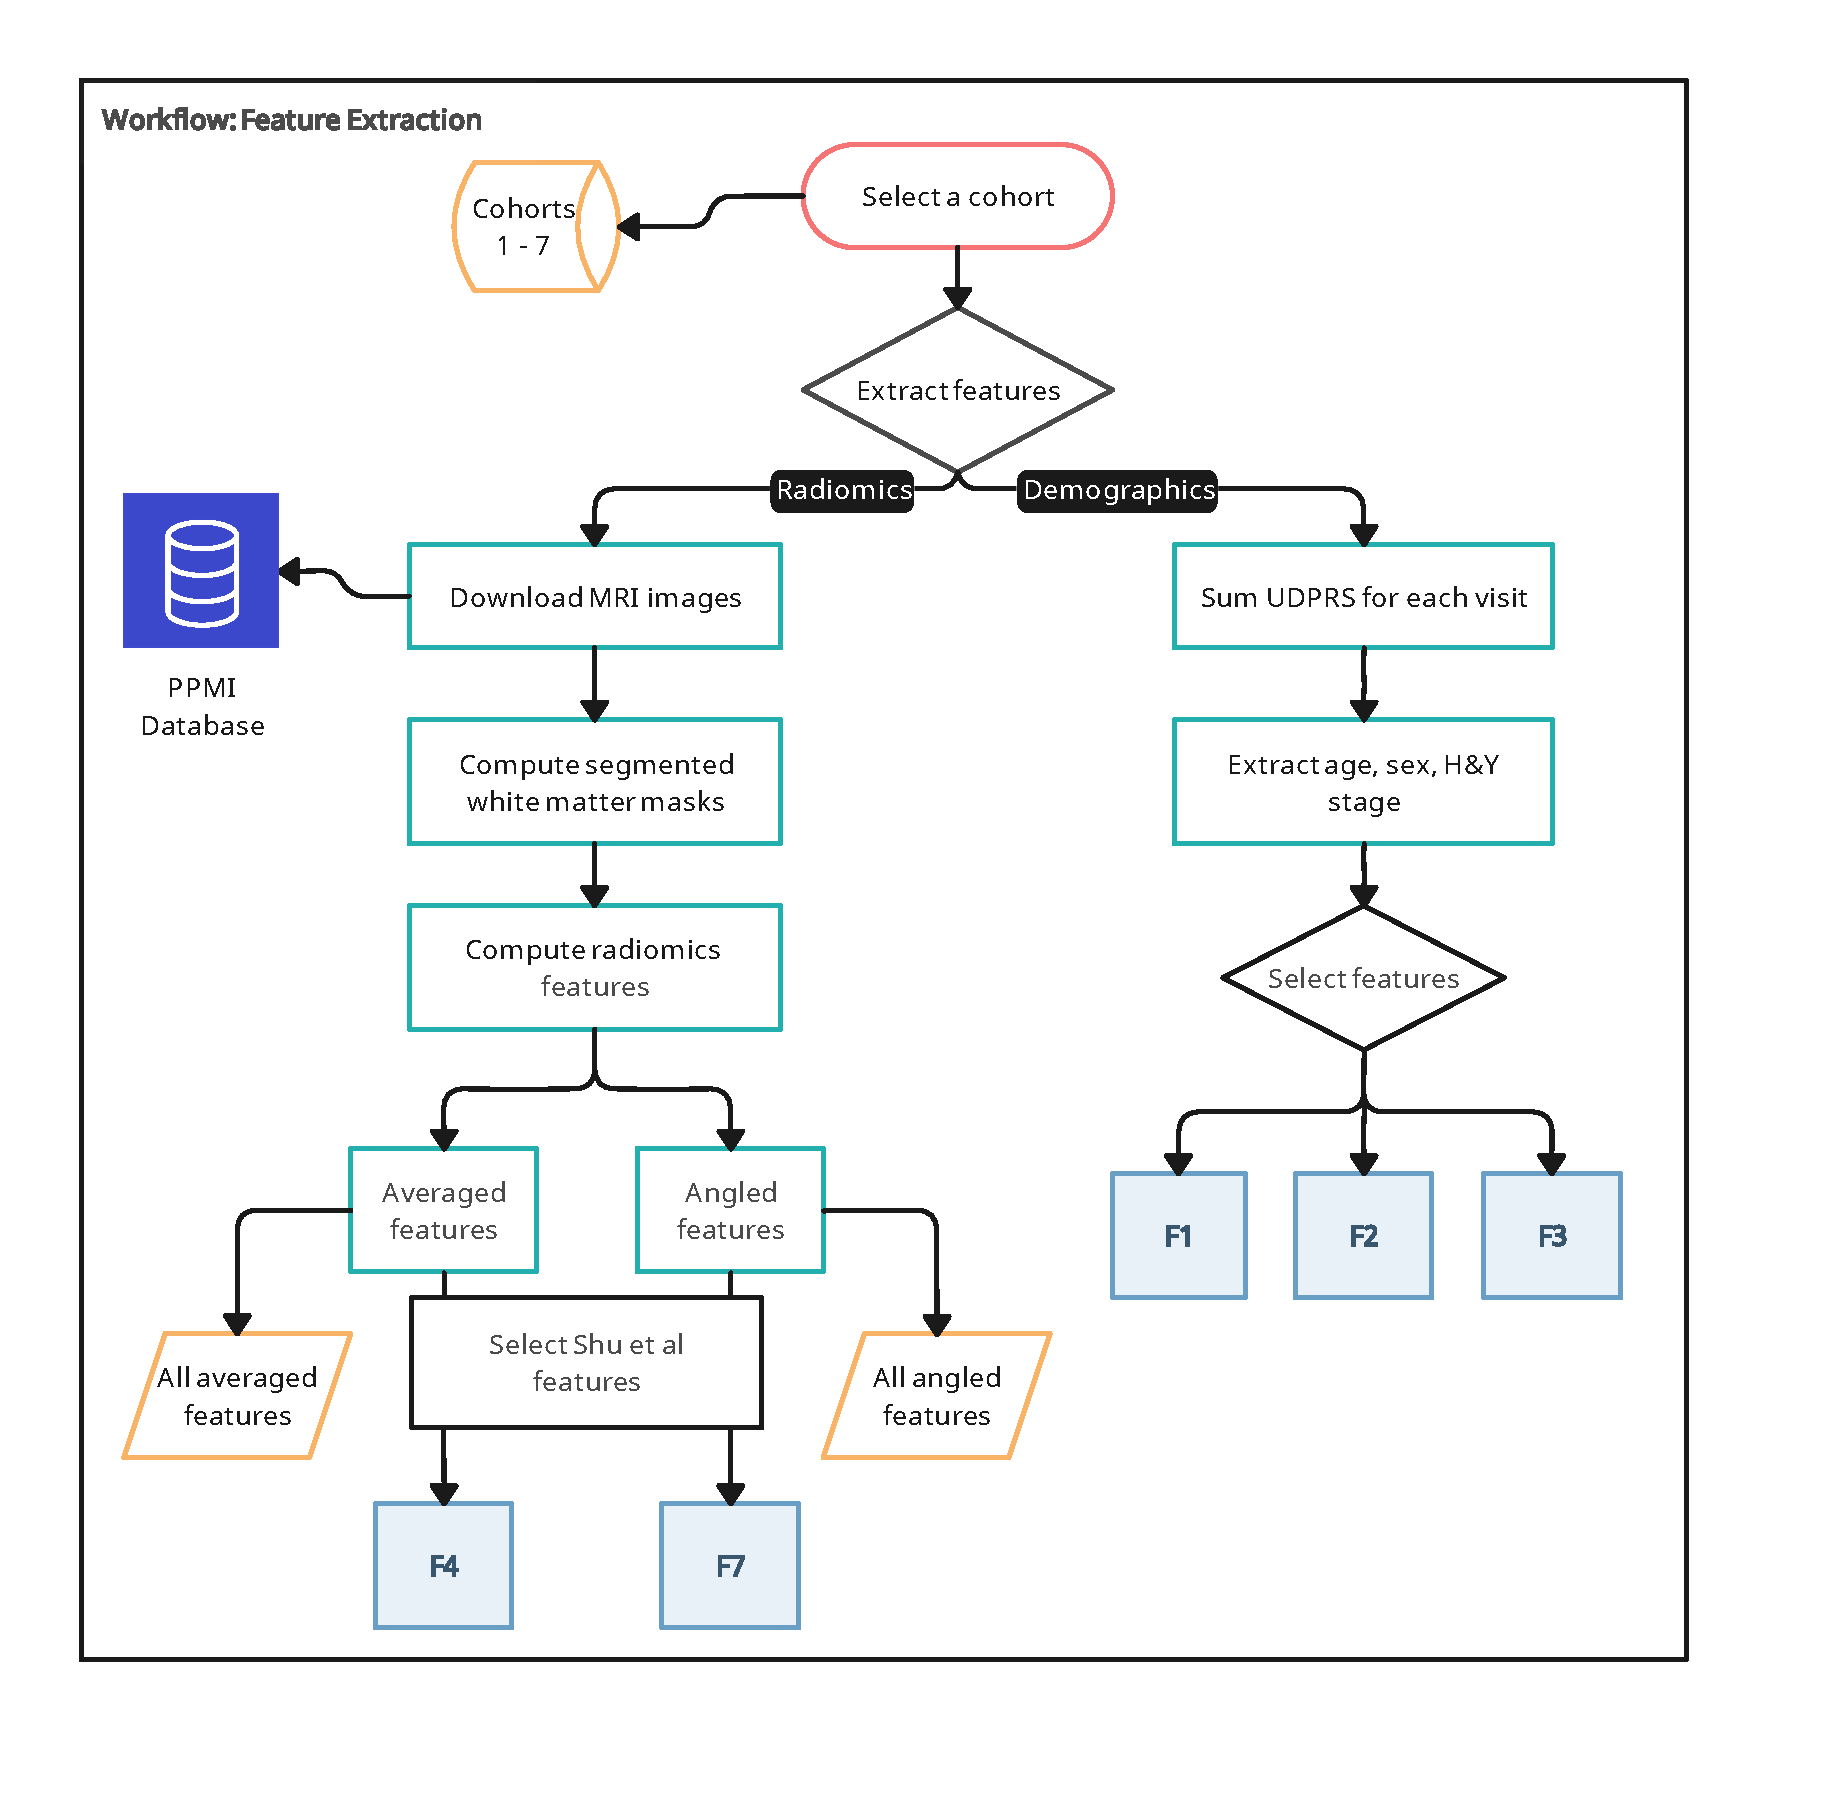
\includegraphics[width=\linewidth]{images/Workflow_feature_extraction.pdf}
  \caption{{\bf Feature Extraction} Extraction of the radiomic and demographic features.}
  \label{featureExtraction}
\end{figure}

\subsubsection*{Demographic features}
Three sets of demographic features were defined:

\begin{itemize}
    \item \textbf{F1}: age, sex, H\&Y score
    \item \textbf{F2}: age, sex, UPDRS total score
    \item \textbf{F3}: age, sex, H\&Y score, UPDRS total score
\end{itemize}


The selection of the age, sex, Unified Parkinson's Disease Rating Scale (UPDRS) total score, and the H\&Y score 
for the demographic features is due to the possibility that they may be contributing factors to whether a subject 
is classified as progressive or stable \TG{this justification needs to be checked with Madeleine}; meaning an imbalanced dataset with respect to these features may impact the results \TG{Any knowledge of data imbalance will impact the results, regardless of the clinical relevance of the features}.  
The demographic features were taken from the first of the selected visits for each subject in the cohorts. While the age, sex, 
and H\&Y score were accessible in the study files from the PPMI database, the Unified Parkinson's Disease Rating Scale (UPDRS) scores 
are derived from a four part assessment of the motor and non-motor functions of a subject~\cite{goetz_tilley_shaftman_stebbins_fahn_martinez-martin_poewe_sampaio_stern_dodel_et_al._2008}. 
The scores from all four parts of the UPDRS assessment were summed to obtain the UPDRS total score.

\subsubsection*{Radiomic features}


In Shu et al., the authors extracted a total of 378 features using A.K. software (Artificial-Intelligent Radio-Genomics Kits; GE Healthcare, Chicago, IL, USA), including 42 histograms features, 10 Haralick features, 9 FormFactor features, 126 GLCM features, 180 GLRLM features, and 11 gray level region matrix features (GLZSM). From these 378 features, the authors used the maximum relevance minimum redundancy (mRMR) algorithm to extract the following top 7 features and train the model:
\begin{itemize}
    \item Feature 1: GLCMEntropy\_AllDirection\_offset1
    \item Feature 2: RunLengthNonuniformity\_angle45\_offset7
    \item Feature 3: Correlation\_angle45\_offset1
    \item Feature 4: HaralickCorrelation\_angle90\_offset4
    \item Feature 5: ShortRunEmphasis\_angle0\_offset7
    \item Feature 6: HaralickCorrelation\_AllDirection\_offset7
    \item Feature 7: Inertia\_AllDirection\_offset4
\end{itemize}

The A.K. software used in Shu et al. is not publicly available. Therefore, we used PyRadiomics~\cite{pyradiomics_2017}, a widely-recognized open-source Python package for the extraction of radiomics features~\cite{Zwanenburg_2020}.
The first set of radiomic features, F4, refer to the set of PyRadiomics features that best match the 7 A.K software features from Shu et al., namely:

\begin{itemize}
    \item Feature 1: Joint Entropy
    \item Feature 2: Run Length Non Uniformity
    \item Feature 3 / Feature 4 / Feature 6: Correlation
    \item Feature 5: Short Run Low Gray Level Emphasis
    \item Feature 7: Contrast
\end{itemize}

For feature sets F5 and F6, we leveraged the entire set of relevant features extracted with PyRadiomics by applying two distinct feature selection techniques: Principal Component Analysis (PCA) for F5 and mRMR for F6. Further details regarding the parameters and implementation of these techniques will be provided in subsequent sections.

The mapping between A.K software and PyRadiomics features is not exact. Indeed, the A.K software, unlike PyRadiomics, provides every feature at a specific angle and offset. In PyRadiomics, for each feature class, the value of a feature is calculated for each angle separately, after which the mean of these values is returned. The exact definitions of these features are available in the PyRadiomics documentation (\url{https://pyradiomics.readthedocs.io/en/latest/features.html}) and in the supplementary material of~\cite{shu2021predicting}, Table S2. 

To address this issue, we extended PyRadiomics to allows users to request features at specific angles and offsets \TG{In a "availability of code" section, add a link to this extension. If possible, PR it to Pyradiomics.}. Using this extension, we were able to construct three additional feature sets. The first of three feature sets, F7, consists of the 7 features found in Shu et al. usign the same offset and angle. F8 and F9 utilize all features extracted at every angle and offset, applying both PCA and MRMR to derive a final set of features. Table ~\ref{table:feature_summary} summarizes the nine feature sets used in our study.

\begin{table}[ht]
  \centering
  \captionof{table}{Summary of the nine feature sets.}
  \begin{tblr}{
    colspec={X[c,1] X[3,l]},
    column{1}={c},
    row{1}={c},
    hlines,
  }
    Feature Set & Summary. \\
    F1 & Patient demographics including age, sex, and H\&Y score. \\
    F2 & Patient demographics including age, sex, and UPDRS score. \\
    F3 & Patient demographics including age, sex, H\&Y score, and UPDRS score. \\
    F4 & PyRadiomics features aligned with Shu et al.'s A.K. Software features. \\
    F5 & PyRadiomics features with PCA feature selection. \\
    F6 & PyRadiomics features with MRMR feature selection. \\
    F7 & Angled PyRadiomics features aligned with Shu et al.'s A.K. Software features. \\
    F8 & Angled PyRadiomics features with PCA feature selection. \\
    F9 & Angled PyRadiomics features with MRMR feature selection. \\
  \end{tblr}
  \label{table:feature_summary}
\end{table}

